%************************************************
\chapter{To control a lamp from two different places}
%************************************************
\begin{flushright}
August 25, 2012
\end{flushright}
\section{Aim}
To control a lamp from two different places.

\section{Theory}
	Two simple circuits can be used for controlling a lamp from two different places. 
	\par
	\autoref{E2_fig1A} shows the first setup, consisting of 2 two way switches (or more precisely, SW-SPDTs, viz. Switch - Single Pole Double Terminal) and a lamp holder. The idea here is to use the two way switches to connect and disconnect the phase of the Lamp holder, while the neutral is hard wired.
	\par
	In \autoref{E2_fig1B}, instead of connecting the neutral permanently to the Lamp holder, we use the fact that the Lamp will be operational, as long as one of the terminals is connected to Phase and the other to Neutral. This configuration, as given in the circuit diagram, is a simple realization of the same.
	\subsection {Tools}
		\begin{enumerate}
			\item Pliers
			\item Screwdriver
			\item Electrical Line Tester
		\end{enumerate}
	\subsection {Material}
		\begin{enumerate}
			\item Two way switches
			\item Lamp
			\item Lamp Holder
			\item Bakelite Sheet
			\item Wires
			\item Screws
			\item Nut Bolts
			\item Terminals
		\end{enumerate}
\section{Procedure}
	\begin{enumerate}
		\item Took a suitable Bakelite sheet and attached the following using screws \& nut-bolts
			\begin{enumerate}
				\item Power Connectors
				\item Switches
			\end{enumerate} 
		\item Connected the circuit according to the circuit diagrams as given in \autoref{E2_fig1A} and \autoref{E2_fig1B}, keeping the following in mind
		\begin{figure}[bth]
			\begin{center}
				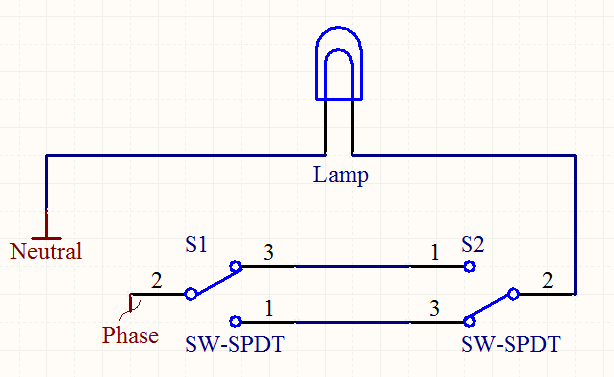
\includegraphics[width=.8\linewidth]{gfx/circuit2_A}
			\end{center}
		\caption[Lamp - 2 Two Way Switch - Method 1]{Lamp controlled by 2 different Two Way Switches}\label{E2_fig1A}
		\end{figure}

		\begin{figure}[bth]
			\begin{center}
				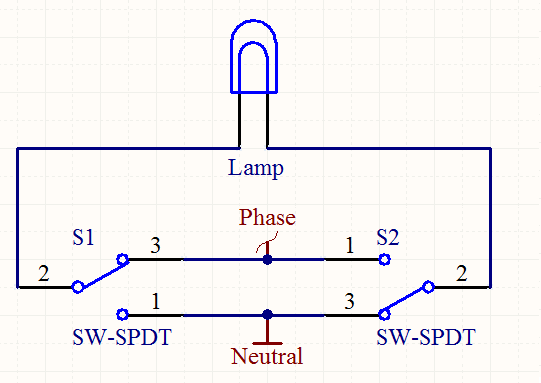
\includegraphics[width=.8\linewidth]{gfx/circuit2_B}
			\end{center}
		\caption[Lamp - 2 Two Way Switch - Method 2]{Lamp controlled by 2 different Two Way Switches}\label{E2_fig1B}
		\end{figure}

			\begin{enumerate}
				\item \emph{Red Wires} are used for the phase connections.
				\item \emph{Black Wires} are used for the neutral connections.
				\item Colours other than Red, Black and Green can be used for the connecting wires.
			\end{enumerate}	
		\item Attached the remaining components using screws \& nut-bolts.			
	\end{enumerate}
\section{Precaution}
	\begin{enumerate}
		\item Connections should be tight, viz. shouldn't come out when pulled.
		\item Wires shouldn't be sticking out of the connections without insulation.
		\item Wires should be of appropriate length.
		\item Colours of the wires should be chosen in accordance with their type.
	\end{enumerate}	
\section{Acknowledgements}
I thank Mr. Jatinder Singh for his guidance during the experiment.